\documentclass[prez_parietal.tex]{subfiles}
\begin{document}


\begin{frame}{Parallel Coordinate Descent}

	Coordinate descent only update one coordinate at each iteration.\\[.5em]
	{\centering {\usebeamercolor[fg]{block title}$\Rightarrow$} Not efficient for convolutional model.\\[1.5em]}
	

	We could update $M$ coefficients in {\bf parallel}.\\[1.5em]
	
	{\bf Existing Parallel Coordinate Descent:}\\
	\begin{itemize}
		\item Synchronous: \cite{Scherrer2012}, \cite{Bradley2011}.
		\item Asynchronous: \cite{Yu2012}, \cite{Low2012}.
	\end{itemize}

	{\bf Can we do better with the structure of our problem?\\[1em]}
	\begin{itemize}
	\item Asynchronous updates
	\item Communication efficient
	\item No exogenous parameters
	\item Large coordinate updates
\end{itemize}

\end{frame}


%---------------------------------------------------------------------------
\subsection{Convolutional Coordinate Descent}
%---------------------------------------------------------------------------

\begin{frame}[t]
\frametitle{Coordinate Descent (CD)}
	
	Minimize
	\[
	Z^{*} = \argmin_{Z}\| X - \sum_{k=1}^K\pmb D_k *  Z_k\|_2^2
			+ \lambda\| Z\|_1
	\]
	Update one coordinate at each iteration.\\[1em]
	\begin{enumerate}
		\item<1-> Select a coordinate $(k_0, t_0)$ to update.
		\item<2-> Compute a new value $Z'_{k_0}[t_0]$ for this coordinate
	\end{enumerate}
	\only<3>{\vskip3em$\Rightarrow$ Converges to the optimal point for CSC problem in $\bO{\frac{1}{q}}$ iterations.}

\only<1>{
	Three algorithms:
	\begin{itemize}\itemindent1em
		\item Cyclic updates; $\bO{1}$  \mycite{Friedman2007}
		\item Random updates; $\bO{1}$ \mycite{Nesterov2010}
		\item Greedy updates; $\bO{KL}$ \mycite{Osher2009}
	\end{itemize}
}
\only<2>{
	For convolutional CD, we can use optimal updates:
	$$
		Z'_{k_0}[t_0] = \frac{1}{\|\pmb D_{k_0}\|_2^2}\text{Sh}(\beta_{k_0}[t_0], \lambda),
	$$
	with {\small $\text{Sh}(y, \lambda) = \text{sign}(y)(|y| - \lambda)_+$}.
	\cite{Kavukcuoglu2013} showed this can be done efficiently, with $\mathcal O(KW)$ operations.
	
	\bimplies{Local operations}
}
\end{frame}


%---------------------------------------------------------------------------
\subsection{DICOD}
%---------------------------------------------------------------------------


\begin{frame}{Distributed Convolutional Coordinate Descent (DICOD)}
	\vskip1em
	
	$Z$ is the coding signal of length $L$.\\[.5em]
	Each core $\mathcal C_m$ is responsible for the updates of a segment
	$\left \{ m \left\lfloor\frac{L}{M}\right\rfloor , \dots
						(m+1) \left\lfloor\frac{L}{M}\right\rfloor -1 \right \}$ .\\[.5em]

	\inputTikZ{.75}{dicod_tikz.tex}
\end{frame}


\begin{frame}{DICOD convergence}


\setbeamercolor{my title}{bg=primary!60, fg=secondary}
\setbeamercolor{my body}{bg=white, fg=black}
%\twocols{
%	\vskip1em
%	\btitle{DICOD, algorithm and convergence result}
%	\vskip1em
%
%    \begin{beamerboxesrounded}[upper=my title,lower=my body,shadow=true]{
%		\usebeamerfont{block title}DICOD pseudo-code}
%	\begin{algorithmic}[1]
%
%		\STATE {\bf Input: }$\pmb D, X$, parameter $\delta >  0$
%		\STATE{ {\bf In parallel } for $m=1\cdots M$}
%		\STATE For all $(k,t)$ in $\mathcal C_m$, initialize $\beta_k[t]$ and $Z_k[t]$%
%		\REPEAT
%		\STATE Receive messages and update $\beta$%
%		\STATE  $\forall (k, t) \in \mathcal C_m$, compute $Z'_k[t]$
%		\STATE Choose $\displaystyle(k_0, t_0) = \arg\max_{(k, t)\in\mathcal C_m} |\Delta Z_k[t]|$
%		\STATE Update $\beta$ and $Z_{k_0}[t_0]\leftarrow{}Z'_{k_0}[t_0]$%
%		\STATE {\bf if}{ $t_0 - mL_M < W$ {\bf then}}
%		\STATE ~~~~Send $(k_0, t_0, \Delta Z_{k_0}[t_0])$ to core $m-1$
%		\STATE {\bf if}{ $(m+1)L_M - t_0< W$ {\bf then}}
%		\STATE ~~~~Send $(k_0, t_0, \Delta Z_{k_0}[t_0])$ to core $m+1$
%		\UNTIL{for all cores, $|\Delta Z_{k_0}[t_0]| < \delta$ }

%	\end{algorithmic}
 %   \end{beamerboxesrounded}
%}{\vskip4em

\begin{beamerboxesrounded}[upper=my title,lower=my body,shadow=true]{
	\usebeamerfont{block title}Theorem (Convergence of DICOD)}
		We consider the following assumptions:\\[.3em]
		{\bf H1: }
		If the cross correlation between atoms of $\pmb D$ is strictly smaller than 1.\\[.3em]
		{\bf H2: }
		No cores stop before all its coefficients are optimal.\\[.3em]
		{\bf H3: }
		If the delay in communication between the processes is inferior to the update time.\\[1em]
		Under these assumptions, the DICOD algorithm converges asymptotically to the
		optimal solution $Z^*$. \mbox{\autoref{eq:sparse_code}}.
	\end{beamerboxesrounded}

\end{frame}


\begin{frame}
	\definecolor{fista}{RGB}{192,192,0}
	\definecolor{rcd}{RGB}{0,128,0}
	\definecolor{cd}{RGB}{255, 0, 0}
	\definecolor{dicod}{RGB}{0,0,255}

		\frametitle{Numerical Experiments}
		Test on long signals generated with Bernoulli-Gaussian
		coding signal $Z$ and a Gaussian dictionary $\pmb D$.
		Fixed $K = 25$, $W = 200$ and $T = 600*W$,\\[1em]
	
	\textbf{Algorithms implemented for benchmark}
	\begin{itemize}
		\item {\color{cd} Coordinate Descent} (CD) \\\mycite{Kavukcuoglu2013}
		\item {\color{rcd} Randomized Coordinate Descent} (RCD) \\\mycite{Nesterov2010}
		\item Fast Convolutional Sparse Coding (FCSC)\\\mycite{Bristow2013}
		\item {\color{fista}Fast Ierative Soft-Thresholding Algorithm (FISTA)} \\\mycite{Chalasani2013, Wohlberg2016}
		\item {\color{dicod} DICOD with $60$ cores}
	\end{itemize}
\end{frame}


\begin{frame}{Numerical convergence}

		\twocols{
			\centering
			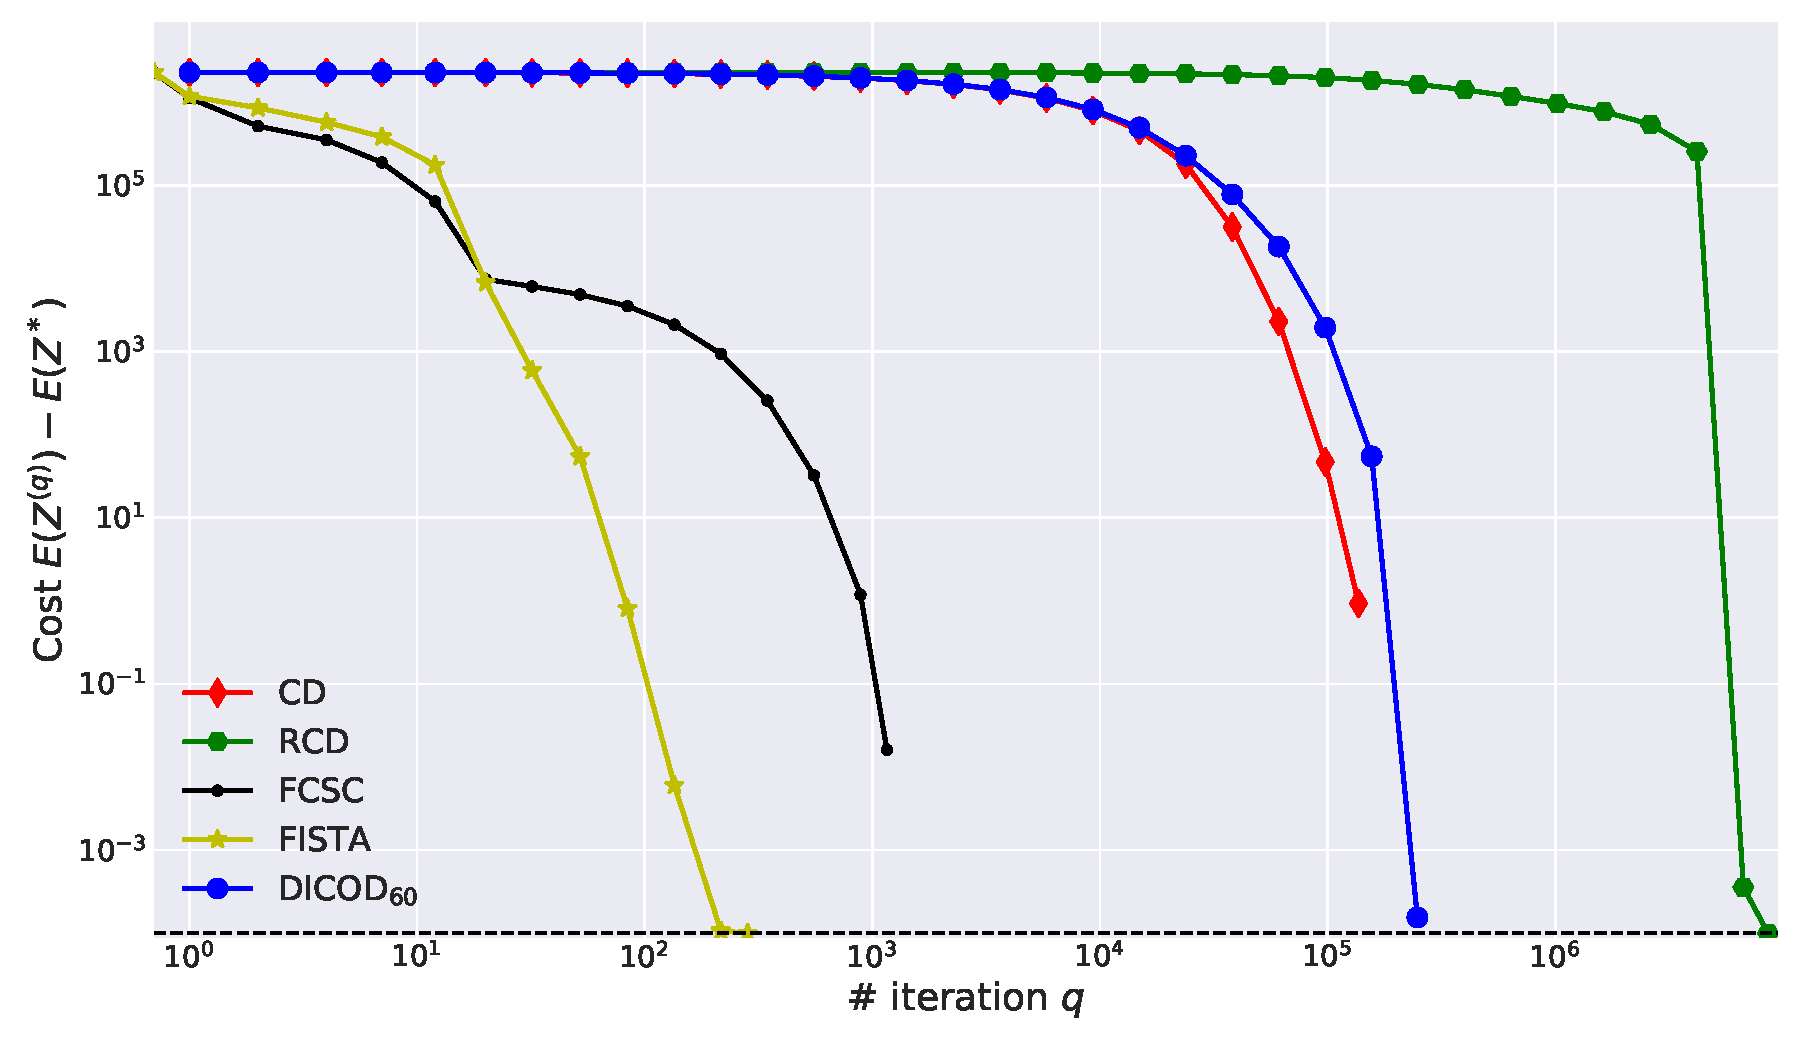
\includegraphics[width=.47\textwidth]{cost_min_seaborn_iter}
			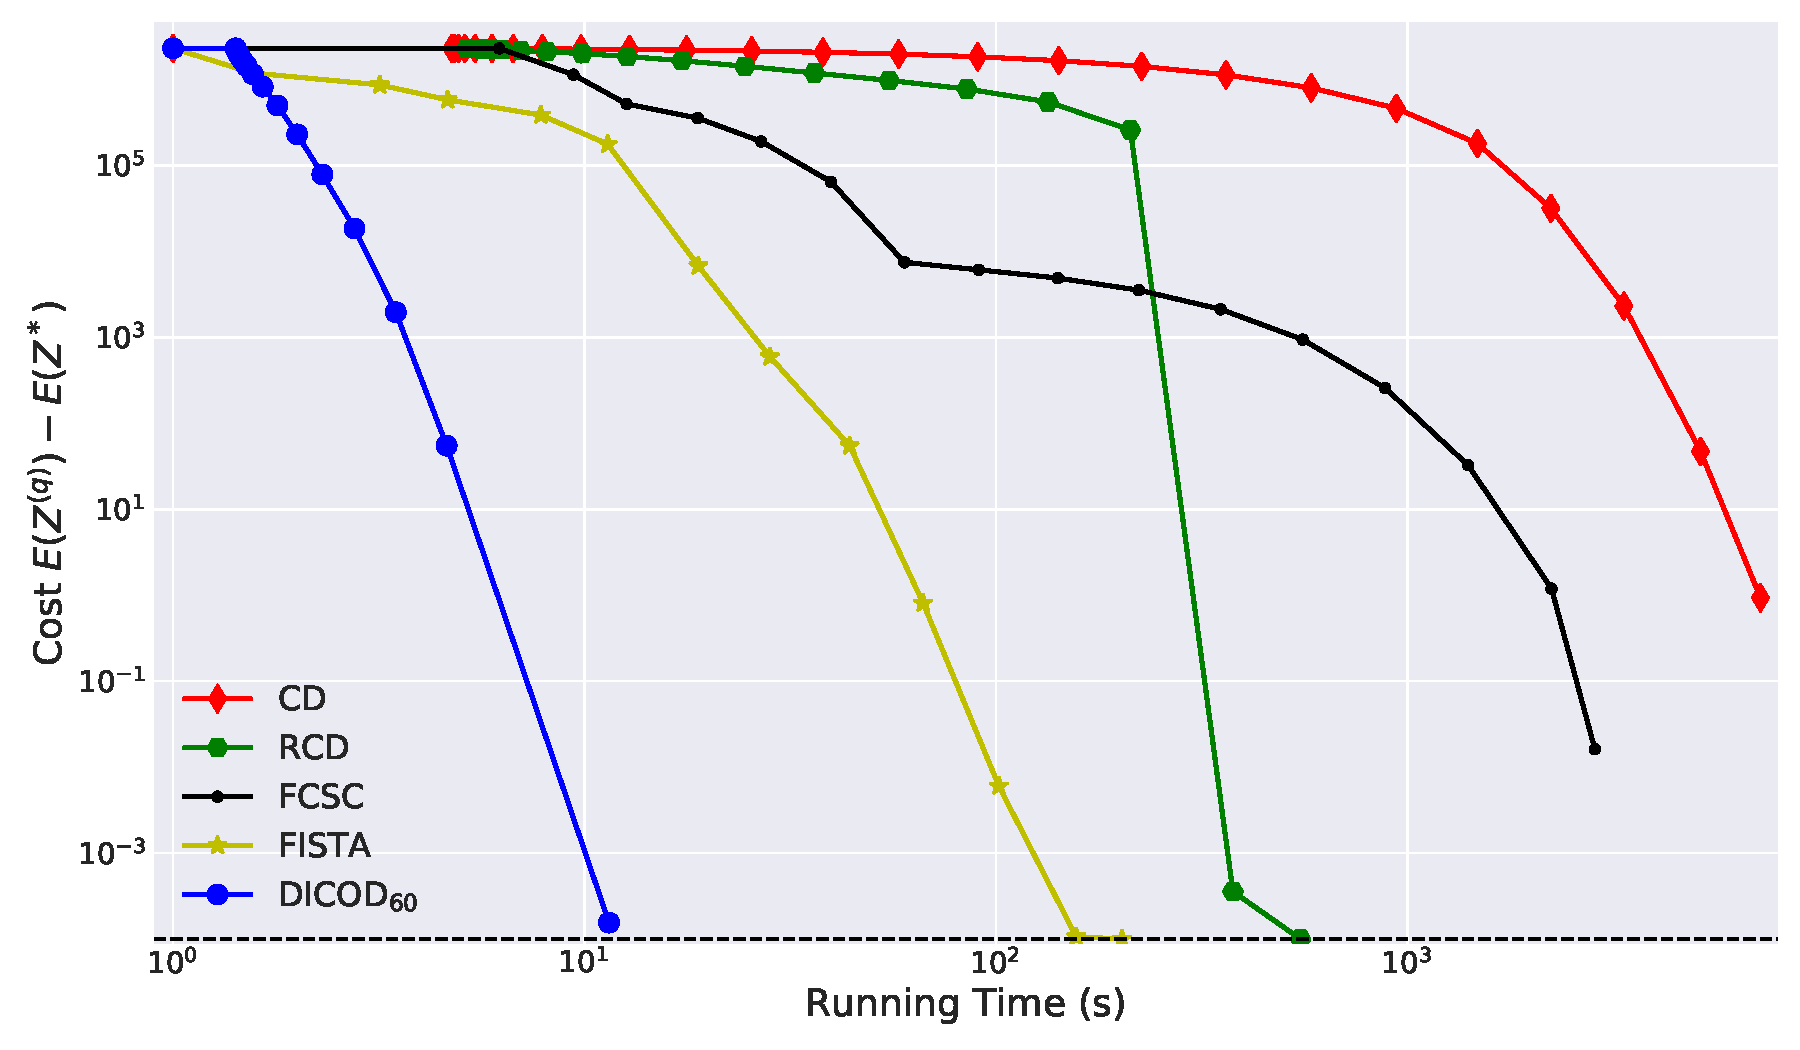
\includegraphics[width=.47\textwidth]{cost_min_seaborn_time}\\
			\large Cost as a function of the iterations Cost as a function of the runtime
		}
\end{frame}


%---------------------------------------------------------------------------
\subsection{Complexity Analysis}
%---------------------------------------------------------------------------

\begin{frame}{Complexity Analysis}
	Two sources of acceleration:\\[1em]
	\begin{itemize}\itemsep1em
		\item Perform $M$ updates in parallel,
		\item Each update is computed on a segment of size $\frac{L}{M}$\\
		Iteration complexity of $\bO{K\frac{L}{M}}$ instead of $\bO{KL}$ 
	\end{itemize}
	\vskip1em
	Limitations:
	\begin{itemize}
	\item Interfering updates, with probability $\alpha^2 = \left(\frac{WM}{T}\right)^2$
	\[
		\mathbb E[Q_{dicod}] \smeq\underset{\alpha \to 0}{\gtrsim}
			M(1-2\alpha^2M^2 + \mathcal O(\alpha^4M^4))~.
	\]
	\item Cost of the update of $\beta$ in $\bO{KW}$  
\end{itemize}

\end{frame}
\begin{frame}{Speed-up of DICOD}
	\centering
	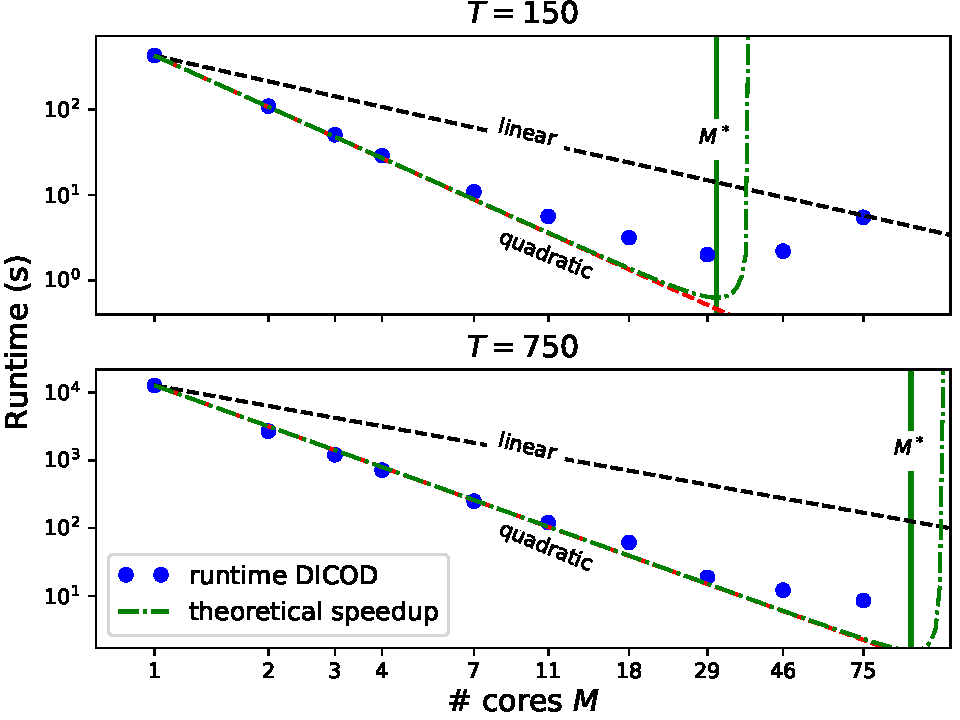
\includegraphics[width=.8\textwidth]{scaling}\\
	\large Runtime as a function of the number of cores $M$
\end{frame}

\begin{frame}{Contributions}

	\twoblocks{Contributions}{\vskip2em
	\begin{itemize}\itemsep.5em
		\item \underline{A novel algorithm DICOD:} distributed algorithm efficient to solve the
		CSC problem,
		\item \underline{Theoretical guarantees:} convergence to the optimal solution,
		\item \underline{Complexity analysis:} achieves a super-linear speedup
	\end{itemize}
	\vskip1.5em
	
	}{Future work}{\vskip2em
	\begin{itemize}\itemsep.5em
		\item Locally greedy coordinate descent
		\item 2D convolutions: extension of this algorithm to images,
		\item Local penalization: extension of this algorithm for localized penalties.
	\end{itemize}
	}
\end{frame}





\biblio{}
\end{document}